\section{Comparateur}

Afin de pouvoir utiliser facilement le signal du micro dans la suite de notre système, nous voudrions que ce signal ne puisse se trouver que dans deux états: soit à une tension nulle (0 V)  soit à la tension d'alimentation $V_{DD}$.  Nous allons donc créer un \textbf{bloc comparateur}. Le résultat attendu à la sortie de celui-ci est donné à la Figure \ref{fig:compare}. Le signal d'entrée (bleu) est comparé à une valeur seuil (rouge): si la valeur du signal d'entrée est plus grande que le seuil, alors la valeur de sortie du comparateur est mise à $V_{DD}$, sinon elle est égale à zéro. 

\begin{figure}[h!]
    \centering
    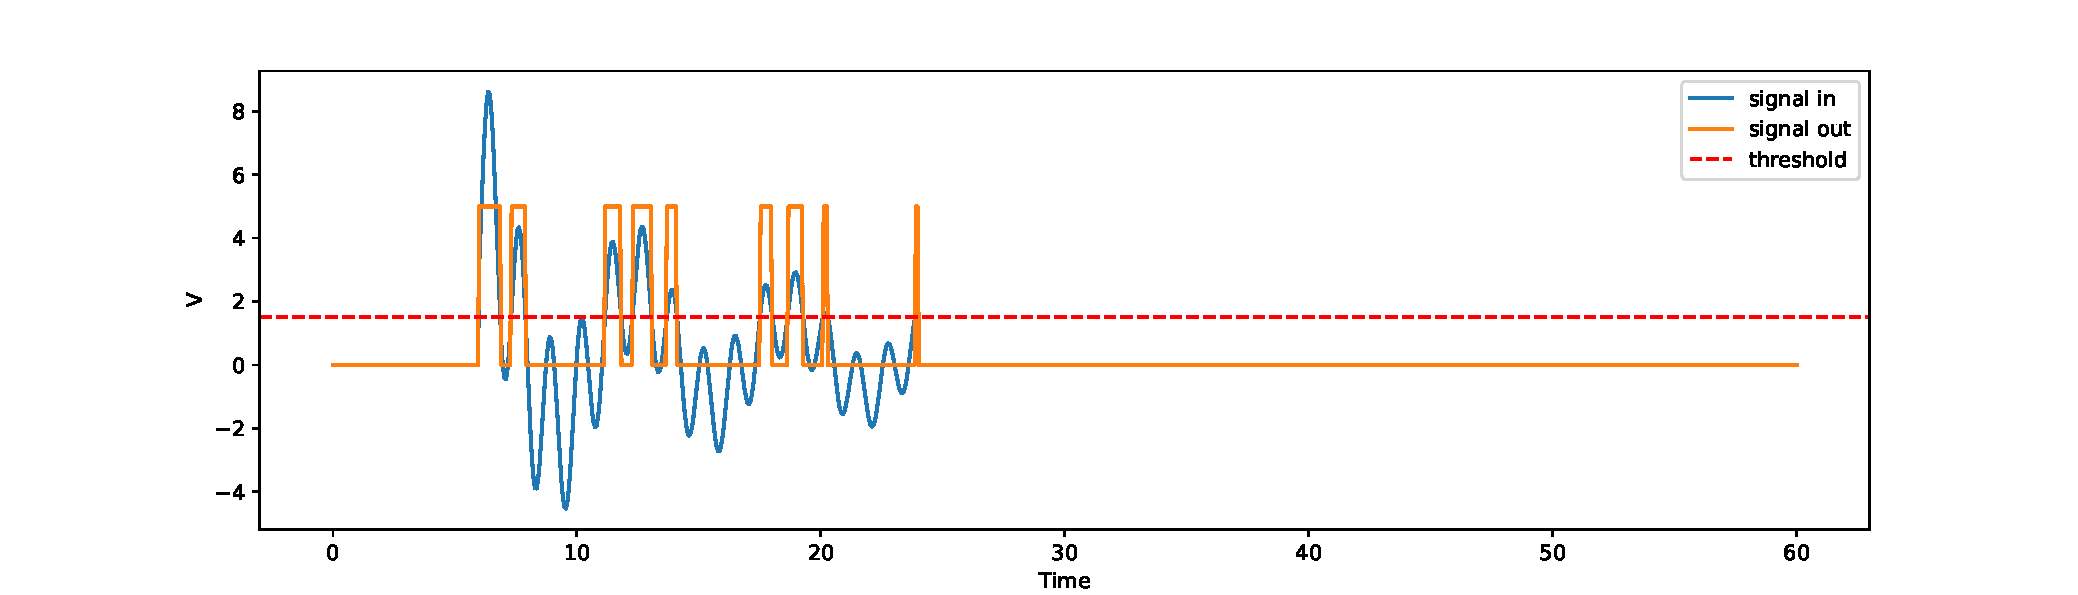
\includegraphics[width=1\linewidth]{figures/club_compare.pdf}
    \caption{Signal à l'entrée et à la sortie d'un comparateur.}
    \label{fig:compare}
\end{figure}

Cette comparaison est réalisée grâce au \texttt{MCP6541} dont le schéma est donné à la Figure \ref{fig:comparecircuit}. Il faut cependant être bien attentif à la manière de connecter les signaux externes à ce petit composant utilisé ici comme une \textit{boîte noire}. Sur sa borne $[+]$, il faut connecter le signal seuil et sur sa borne $[-]$, le signal d'entrée. Le signal seuil est fixé par le designer grâce à un \textbf{diviseur résistif} composé de $R_3$ et de $R_4$. Ces équations sont données par

\begin{equation}
    V_{DD} = V_{R_3} + V_{R_4}  = I*(R_3 + R_4) \quad \text{mais aussi} \quad V_{R_4} = V_{seuil} =  I*R_4,
\end{equation}
et donc
\begin{equation}
    V_{seuil} = V_{DD} \frac{R_4}{R_3+R_4}. \\
\end{equation}

\vspace{0.3cm}

La valeur du seuil est donc donnée en fonction de $V_{DD}$, $R_3$ et $R_4$. La tension $V_{DD}$ est fixée à $5$[V]. Pour ce qui est des résistances, nous vous proposons d'utiliser $R_3=100$[$\Omega$]. La résistance $R_4$ est un potentiomètre ce qu'il signifie que c'est une résistance variable. Vous pouvez donc la modifier pour changer la tension de seuil. Il est intéressant de se poser la question de l'effet de la modification de cette tension de seuil sur l'ensemble du système. Avez-vous une idée ?

\vspace{0.5cm}
\begin{figure}[h!]
    \centering
    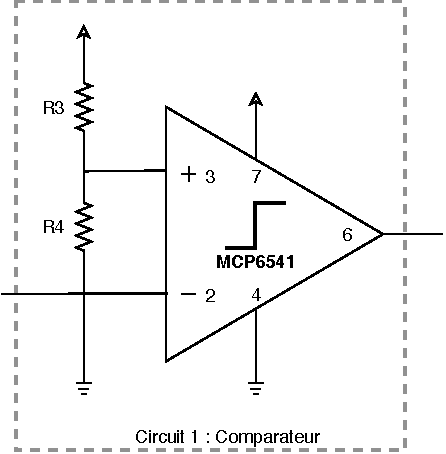
\includegraphics[width=0.5\linewidth]{HO2_comp.pdf}
    \caption{Montage comparateur.}
    \label{fig:comparecircuit}
\end{figure}